
\begin{figure}
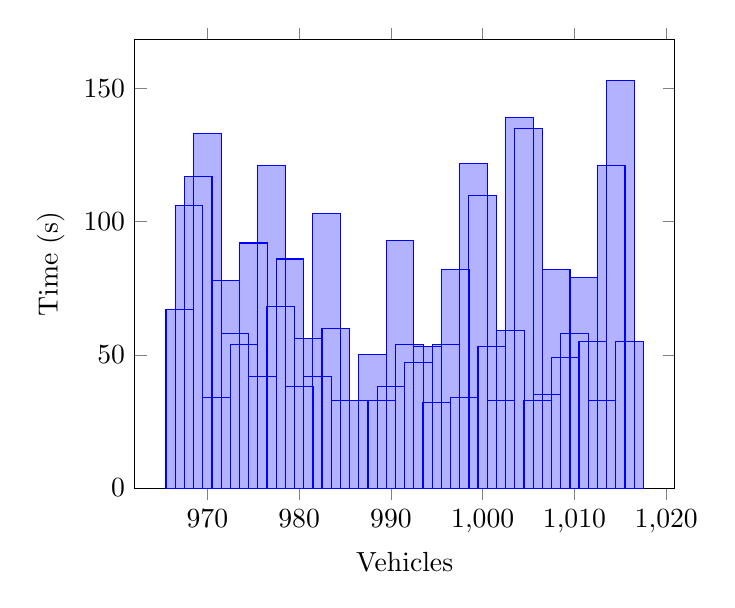
\begin{tikzpicture}
\begin{axis}[
legend style={anchor=west},
xlabel=Vehicles,
ylabel=Time (s),
ymin=0,
ybar,
]
\addplot coordinates {
(994, 53)
(974, 54)
(985, 33)
(977, 121)
(987, 33)
(969, 117)
(1005, 135)
(1000, 110)
(1010, 58)
(993, 47)
(1007, 35)
(972, 78)
(976, 42)
(979, 86)
(1016, 55)
(968, 106)
(1015, 153)
(1003, 59)
(997, 82)
(1014, 121)
(990, 38)
(1012, 55)
(980, 38)
(971, 34)
(995, 32)
(1013, 33)
(988, 50)
(998, 34)
(999, 122)
(992, 54)
(970, 133)
(996, 54)
(1009, 49)
(1002, 33)
(986, 33)
(984, 60)
(982, 42)
(1001, 53)
(983, 103)
(1008, 82)
(989, 33)
(975, 92)
(1011, 79)
(1004, 139)
(973, 58)
(1006, 33)
(967, 67)
(991, 93)
(978, 68)
(981, 56)
};

\end{axis}
\end{tikzpicture}
\label{tik:time:100:89}
\caption{100 percent diving with GSC on route $89$}
\end{figure}
